\documentclass[10pt,twocolumn,letterpaper]{article}

% \usepackage{iccv}
\usepackage{hyperref}  
\usepackage{times}
\usepackage{epsfig}
\usepackage{graphicx}
\usepackage{amsmath}
\usepackage{amssymb}
\usepackage[pagebackref=true,breaklinks=true,letterpaper=true,colorlinks,bookmarks=false]{hyperref}
\usepackage{hyperref}
\usepackage{xcolor}
\usepackage{float}  % Ensures figures stay in place
\usepackage{caption}



\usepackage{xurl}  % Allows better URL handling

\hypersetup{
    colorlinks=true,
    linkcolor=black,
    urlcolor=blue
}
\iccvfinalcopy 

\ificcvfinal\pagestyle{empty}\fi

\begin{document}
\raggedbottom  % Prevents excessive spacing between sections

%%%%%%%%% TITLE
\title{Brain Tumor Classification using MRI Scans}

\author{Lam Nguyen\\
University of Central Florida\\
{\tt\small la815794@ucf.edu}
\and
Faramarz Aboutalebi\\
University of Central Florida\\
{\tt\small fa423345@ucf.edu}
}

\maketitle
\ificcvfinal\thispagestyle{empty}\fi

\begin{abstract}
Effective treatment requires precise classification of brain tumor type because different brain tumors vary in severity and types. Moreover, accurate classification and timely detection can help improve patient outcome. The objective of this project is to design and implement a deep learning based classification model able to distinguish between glioma, meningioma, pituitary tumors, and non-tumor MRI images. For this purpose, we are going to use pre-trained Convolutional Neural Networks ResNet and Vision Transformers to achieve better results. The dataset for this project will be the already existing public Brain MRI dataset on Kaggle because it contains labeled MRI scans that are used for training and evaluation. This project seeks to improve classification accuracy and provide useable explainability with techniques like Grad-CAM.
\end{abstract}

\section{Statement of the Problem}
Classification of brain tumors is a major issue in medical imaging. Given an MRI scan as an input, our system attempts to predict if the image falls under any one of these tumor categories: glioma, meningioma, pituitary tumor, or no tumor.

The motivation stems from the fact that there is a need to assist radiologist by enhancing the speed and accuracy of computerized tumor diagnosis. Traditional methods of diagnosis are usually performed by manual inspection which can take a lot of time and can be subjected to human mistakes.

Using deep learning, we strive to increase both the efficiency and accuracy of this process through automation.

The aim of this project is to create a classification model that can delineate the types of brain tumors with high accuracy, as depicted in the public MRI datasets provided alongside the model. The advanced techniques of deep learning will be utilized to accomplish this objective.

\begin{figure}[H]
    \centering
    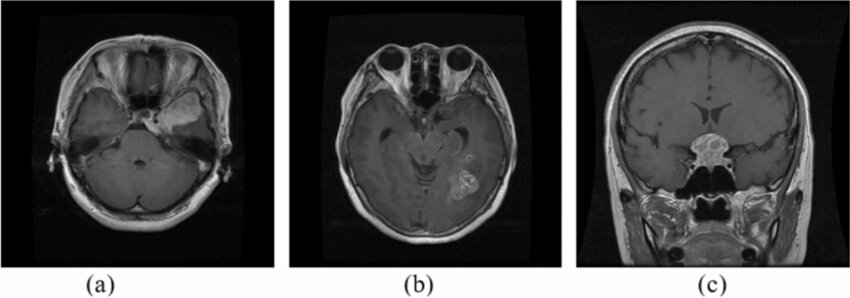
\includegraphics[width=0.9\linewidth]{MRI-images-of-three-different-brain-tumors-a-meningioma-b-glioma-and-c-pituitary.png}
    \caption{MRI images of different brain tumors: meningioma, glioma, and pituitary tumor. Source: ResearchGate.}
    \label{fig:brain_tumor_types}
\end{figure}


\section{Related Work}
The deep learning boom has brought about a new epoch in medical image classification. Previous studies have demonstrated that the CNN architectures such as ResNet, VGG16, and MobileNet have greatly succeeded in various medical imaging tasks.

The rest of the machine learning techniques like SVMs, Random Forests, etc. have also been utilized, but CNN-based models perform the best as they automatically extract features from images.

Newer studies put forth the issue of explainability in medical diagnosis using AI. Models can be made more interpretable with techniques like Grad-CAM, which draw attention to areas of interest to the model and the decisions they affect.

\section{Technical Approach}
Our approach relies on the training and fine-tuning of deep learning models directed towards the classifcation of brain tumors on MRI images.
The preliminary steps are as follows:

\begin{itemize}
    \item \textbf{Data Preprocessing}: During this stage, images are resized to a fixed value of 224 by 224 for CNNs, pixels are normalized, and image augmentation is performed.
    \item \textbf{Model Selection}: Construct a CNN based model ResNet50 or VGG16 and benchmark it against classification by Vision Transformers.
    \item \textbf{Transfer Learning}: With the help of existing models, training time can be decreased while increasing accuracy.
    \item \textbf{Model Evaluation}: Train the models on the Kaggle dataset and determine performance of the models through evaluation metrics such as accuracy, precision, recall, and F1 score.
    \item \textbf{Explainability}: Have Grad-CAM show how the model arrived at a decision.
\end{itemize}

\begin{figure}[H]
    \centering
    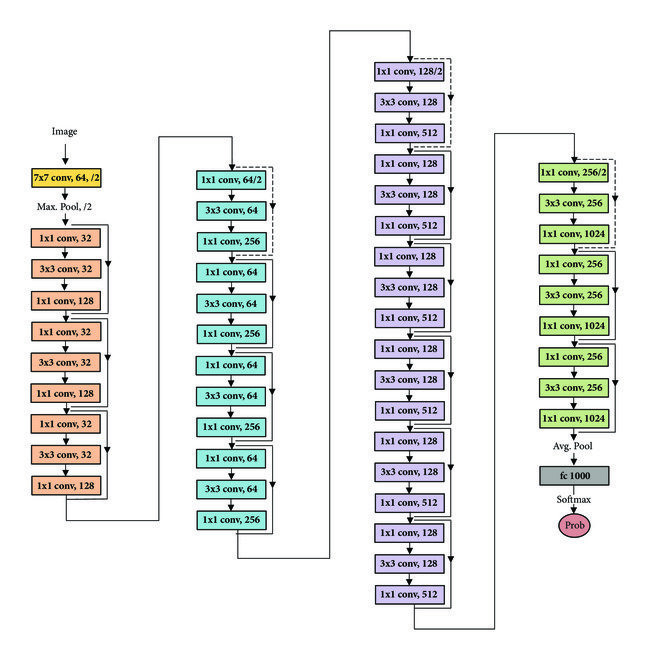
\includegraphics[width=0.9\linewidth]{Block-diagram-of-Resnet-50-1-by-2-architecture.png}
    \captionsetup{aboveskip=2pt, belowskip=2pt} % Reduces space above and below the caption
    \caption{Block diagram of ResNet-50 architecture. Source: ResearchGate.}
    \label{fig:resnet_architecture}
\end{figure}




\section{Experiments}
We will:
\begin{itemize}
    \item Participate in the classification competition by training the aforementioned CNN architectures ResNet50, MobileNet, Vision Transformers, and analyzing their performance.
    \item Test the implementation of classification image augmentation techniques and measure changes in accuracy.
    \item Use various indicators of model performance such as accuracy, F1 score, and confusion matrix.
    \item Conduct Grad-CAM explainability analysis to determine important areas of the images that led the model to make the decision.
\end{itemize}

\begin{figure}[H]
    \centering
    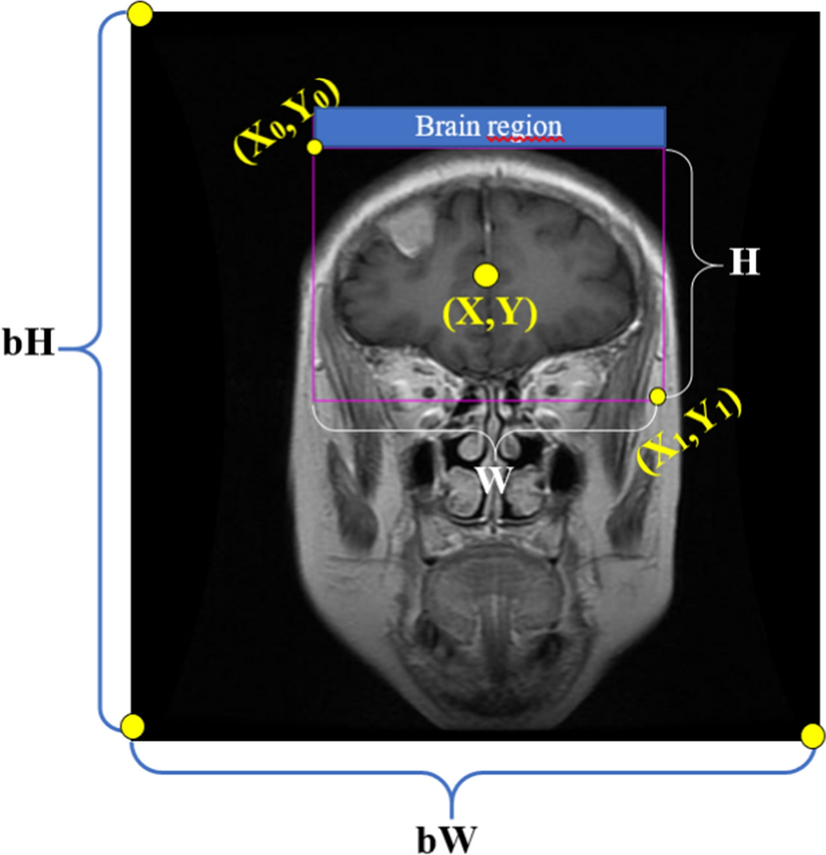
\includegraphics[width=0.9\linewidth]{Coordinate-information-calculated-on-the-labeled-brain-image.png}
    \captionsetup{aboveskip=2pt, belowskip=2pt} % Reduces space above and below the caption
    \caption{Grad-CAM visualization of a brain MRI. Source: ResearchGate.}
    \label{fig:grad_cam_example}
\end{figure}




\textbf{Dataset:} We will use the Brain MRI dataset from Kaggle, which contains labeled images of gliomas, meningiomas, pituitary tumors, and non-tumor MRIs. The dataset is structured into training and testing folders with categorized subdirectories.





\section*{References}
\begin{enumerate}
    \item Deep Learning for Brain Tumor Classification, Kaggle Dataset.  
    \href{https://www.kaggle.com/datasets/navoneel/brain-mri-images-for-brain-tumor-detection}{\nolinkurl{https://www.kaggle.com/datasets/navoneel/brain-mri-images-for-brain-tumor-detection}}
    
    \item He, K., Zhang, X., Ren, S., & Sun, J. (2016). "Deep Residual Learning for Image Recognition." CVPR 2016.  
    \href{https://arxiv.org/abs/1512.03385}{\nolinkurl{https://arxiv.org/abs/1512.03385}}
    
    \item Dosovitskiy, A., et al. (2020). "An Image is Worth 16x16 Words: Transformers for Image Recognition at Scale." ICLR 2021.  
    \href{https://arxiv.org/abs/2010.11929}{\nolinkurl{https://arxiv.org/abs/2010.11929}}
\end{enumerate}




\end{document}
